\documentclass[polish,a4paper]{article}
\usepackage{amsmath}
\usepackage{amssymb, amsfonts, amsthm, amsmath, bm}
\usepackage[T1]{fontenc}
\usepackage[utf8]{inputenc}
\usepackage{babel}
\usepackage{pslatex}
\usepackage{pgfplots}
\usepackage{hhline}
\usepackage[american]{circuitikz} 
\usepackage{anysize}
\usepackage{gensymb}
\usepackage{graphicx}
\DeclareGraphicsExtensions{.jpg}
\marginsize{2.5cm}{2.5cm}{3cm}{3cm}
\bibliographystyle{IEEEtran}


%makro do indeksów w tabeli
\newcommand{\PRzFieldDsc}[1]{\sffamily\bfseries\scriptsize #1}

%makro do informacji w tabeli
\newcommand{\PRzFieldCnt}[1]{\itshape #1}

%potężne makro tworzące tabelę z informacjami o teamie
\newcommand{\PRzHeading}[8]{
%% #1 - nazwa laboratorium
%% #2 - kierunek 
%% #3 - specjalność 
%% #4 - rok studiów 
%% #5 - symbol grupy lab.
%% #6 - temat 
%% #7 - numer lab.
%% #8 - skład grupy ćwiczeniowej

\begin{center}
\begin{tabular}{ p{0.32\textwidth} p{0.15\textwidth} p{0.15\textwidth} p{0.12\textwidth} p{0.12\textwidth} }

  &   &   &   &   \\
\hline
\multicolumn{5}{|c|}{}\\[-1ex]
\multicolumn{5}{|c|}{{\LARGE #1}}\\
\multicolumn{5}{|c|}{}\\[-1ex]

\hline
\multicolumn{1}{|l|}{\PRzFieldDsc{Kierunek}}	& \multicolumn{1}{|l|}{\PRzFieldDsc{Specjalność}}	& \multicolumn{1}{|l|}{\PRzFieldDsc{Rok studiów}}	& \multicolumn{2}{|l|}{\PRzFieldDsc{Symbol grupy lab.}} \\
\multicolumn{1}{|c|}{\PRzFieldCnt{#2}}		& \multicolumn{1}{|c|}{\PRzFieldCnt{#3}}		& \multicolumn{1}{|c|}{\PRzFieldCnt{#4}}		& \multicolumn{2}{|c|}{\PRzFieldCnt{#5}} \\

\hline
\multicolumn{4}{|l|}{\PRzFieldDsc{Temat Laboratorium}}		& \multicolumn{1}{|l|}{\PRzFieldDsc{Numer lab.}} \\
\multicolumn{4}{|c|}{\PRzFieldCnt{#6}}				& \multicolumn{1}{|c|}{\PRzFieldCnt{#7}} \\

\hline
\multicolumn{5}{|l|}{\PRzFieldDsc{Skład grupy ćwiczeniowej oraz numery indeksów}}\\
\multicolumn{5}{|c|}{\PRzFieldCnt{#8}}\\

\hline
\multicolumn{3}{|l|}{\PRzFieldDsc{Uwagi}}	& \multicolumn{2}{|l|}{\PRzFieldDsc{Ocena}} \\
\multicolumn{3}{|c|}{\PRzFieldCnt{\ }}		& \multicolumn{2}{|c|}{\PRzFieldCnt{\ }} \\

\hline
\end{tabular}
\end{center}
}
%koniec potężnego makro do tabeli

\begin{document}

%stworzenie tabeli - miejsce na zmienianie danych w tabeli
%indeksy do uzupełnienia
\PRzHeading{Laboratorium Podstaw Elektroniki}{Informatyka}{--}{I}{I1}{Układy wzmacniaczy operacyjnych}{6}{Ewa Fengler(132219), Sebastian Maciejewski(132275), Jan Techner(132332)}{}

%ZADANIA

\section*{Cel}
Celem przeprowadzanych doświadczeń jest poznanie funkcji wzmacniaczy operacyjnych w układach elektronicznych. \newline

Wszystkie elementy rezystancyjne i pojemnościowe zamieszczone na płycie laboratoryjnej zostały przedstawione w poniższej tabeli :
\begin{table}[!h]
\centering
\begin{tabular}{|r|c|c|c|}
\hline
\textbf{Element obwodu} &\textbf{Oznaczenie} &\textbf{Odczyt} \\ \hline
 \textbf{R\textsubscript{1}} & Brązowy, Czarny, Czerwony, Złoty & 1k$\Omega \pm 5\%$ \\ \hline
\textbf{R\textsubscript{2}} & Brązowy, Czarny, Czerwony, Złoty & 1k$\Omega \pm 5\%$\\ \hline
\textbf{R\textsubscript{3}} & Brązowy, Czarny, Czerwony, Złoty & 1k$\Omega \pm 5\%$\\ \hline
\textbf{R\textsubscript{4}} & Czerwony, Czarny, Czerwony, Złoty & 2k$\Omega \pm 5\%$\\ \hline
\textbf{R\textsubscript{5}} & Brązowy, Czarny, Czerwony, Złoty & 1k$\Omega \pm 5\%$\\ \hline
\textbf{R\textsubscript{6}} & Zielony, Brązowy, Czerwony, Złoty & 5.1k$\Omega \pm 5\%$\\ \hline
\textbf{R\textsubscript{7}} & Brązowy, Czarny, Czerwony, Złoty & 1k$\Omega \pm 5\%$\\ \hline
\textbf{R\textsubscript{8}} & Czerwony, Czarny, Czerwony, Złoty & 2k$\Omega \pm 5\%$\\ \hline
\textbf{C\textsubscript{1}} & 104 & 100$\mu$F\\ \hline
\textbf{C\textsubscript{2}} & 10$\mu$F & 10$\mu$F\\ \hline
\end{tabular}
\caption{Odczytane wartości elementów układu}
\label{fig:pomiary}
\end{table}
\section{Zadanie 1.3}
Badanie działania wzmacniacza w konfiguracji nieodwracającej. 
\subsection*{1.}
Płyta ćwiczeniowa do badania wzmacniacza w konfiguracji nieodwracającej została przygotowana zgodnie ze schematem podanym na stronie\cite{rlc}.  Wartości elementów rezystancyjnych \textbf{R\textsubscript{1}} oraz \textbf{R\textsubscript{2}} odpowiedzialnych za wyznaczanie stopnia wzmocnienia w tej konfiguracji przedstawiono w tabeli \ref{fig:pomiary}.
\subsection*{5.}
Na wyjściu generatora został ustawiony przebieg sinusoidalny o częstotliwości 4kHz, ponieważ taka wartość została podana przez prowadzącego zajęcia.
\subsection*{6.}
Odczytane z oscyloskopu amplitudy przebiegów wejściowych i wyjściowych to : 
\begin{center}
Amplituda przebiegu wejściowego = $\sim$ 0.5V \\
Amplituda przebiegu wyjściowego = $\sim$ 1V
\end{center}
 
\subsection*{7.}
\begin{figure}[!h]
\centering
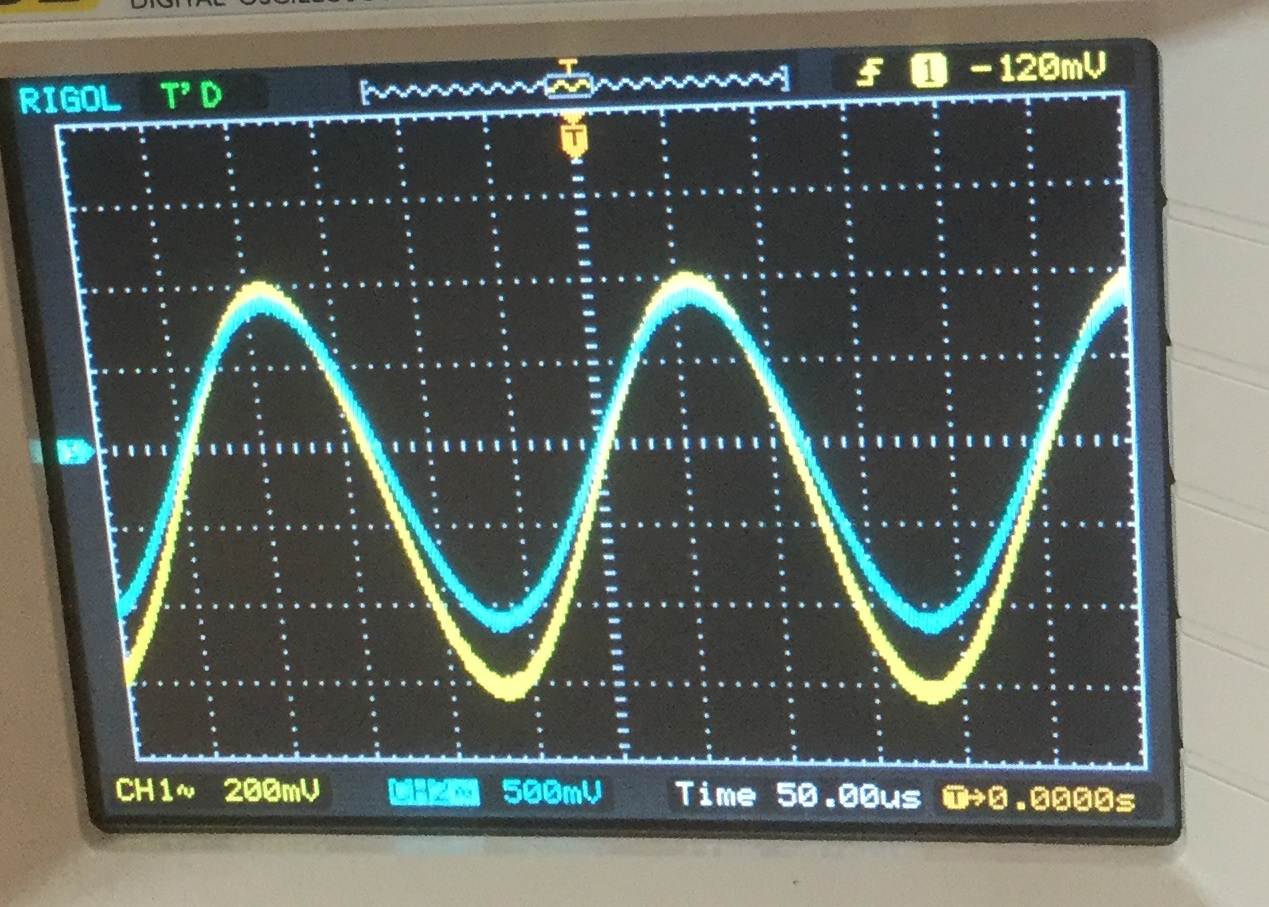
\includegraphics[width=0.5\textwidth]{amplituda}
\caption{oscylogram ukazujący działanie stopnia wzmacniającego w konfiguracji nieodwracającej}
\end{figure}
\subsection*{8.}
$$\frac{A_{out}}{A_{in}} = \frac{1V}{0.5V} = 2$$\\
$$10 log_{10}(2)^2 = 20 log_{10}(2) = 6.02dB$$\\
Oszacowane wzmocnienie wzmacniacza wynosi w skali liniowej $\sim$2[V/V], natomiast w skali decybelowej jest to około 6 dB. \\
\subsection*{9.}
\begin{equation}
\frac{U_{out}(s)}{U_{in}(s)} = 1 + \frac{Z_{f}}{Z_{in}}
\end{equation}
$$\frac{U_{out}(s)}{U_{in}(s)} = 1 + \frac{1k\Omega}{1k\Omega} = 1+1=2$$
$$\frac{U_{out}(s)}{U_{in}(s)} = 2$$
Uzyskana wartość wzmocnienia obliczona w podpunkcie 8 (w skali liniowej) pokrywa się z wartością wzmocnienia obliczoną na podstawie zależności (1)\cite{rlc}
\subsection*{10.}
W układzie wtórnika $Z_f$ wynosi $0\Omega$, a $Z_{in}$ wynosi $\infty$ . Po podstawieniu do wzoru otrzymujemy wartość wzmocnienia równą 1. Wtórnik napięciowy stosuje się w celu separacji wejścia od wyjścia, bowiem nie obciąża on układu wejściowego (generującego napięcie wejściowe), ponieważ impedancja wejściowa wzmacniacza operacyjnego teoretycznie jest nieskończona. Równocześnie, ponieważ teoretyczna impedancja wyjściowa wzmacniacza operacyjnego wynosi 0, w związku z czym może być (teoretycznie) dowolnie obciążona.

\section{Zadanie 1.4}
Badanie działania wzmacniacza w konfiguracji odwracającej. 
\subsection*{1.}
Płyta ćwiczeniowa do badania wzmacniacza w konfiguracji odwracającej została przygotowana zgodnie ze schematem podanym na stronie\cite{rlc}.  Wartości elementów rezystancyjnych oraz pojemnościowych  możliwych do załączenia w roli impedancji Z\textsubscript{f} oraz Z\textsubscript{in} w tej konfiguracji przedstawiono w tabeli \ref{fig:pomiary}.
\subsection*{3.}
Na wyjściu generatora został ustawiony przebieg sinusoidalny o częstotliwości 4kHz, ponieważ taka wartość została podana przez prowadzącego zajęcia.
\subsection*{4.}
W tabeli poniżej zostały umieszczone następujące dane : 
\begin{itemize}
\item teorytyczne wartości wzmocnienia napięciowego $k_u$ obliczone ze wzoru $\frac{U_{out}(s)}{U_{in}(s)} = - \frac{Z_{f}}{Z_{in}}$ \cite{rlc}.
\item amplitudy przebiegów wejściowych $u_{we}$ i wyjściowych $u_{wy}$ dla różnych nastaw Zf oraz Zin odczytane z oscyloskopu.
\item  aktualne wartości wzmocnienia napięciowego $k_u$ układu obliczone na podstawie stosunku $u_{wy}$ i $u_{we}$ wyrażone w skali liniowej i decybelowej.
\end{itemize}

\begin{table}[!h]
\centering
\begin{tabular}{|c|c|c|c||c|c|c|c|c|}
\hline
\textbf{$Z_{in}$} & \textbf{nr przełącznika} & \textbf{$Z_f$} & \textbf{nr przełącznika} & \textbf{$k_u$ teoretyczne } & \textbf{$u_{we}$} & \textbf{$u_{wy}$} & \textbf{$k_u$ [V/V]} & \textbf{$k_u$ [dB] } \\ 
\hhline{|=|=|=|=#=|=|=|=|=|}
$1k\Omega$ & 1 & $2k\Omega$ & 1 & -2 [V/V] & 0,5 V & 1V & 2 & 6.02\\
\hline
$1k\Omega$ & 1 & $1k\Omega$ & 2 & -1 [V/V] & 0,5 V & 0,5V & 1 & 0\\
\hline
$1k\Omega$ & 1 & $5.1k\Omega$ & 3 & -5,1[V/V] & 100mV & 0,5V & 5 & 13.97\\
\hline
$2k\Omega$ & 2 & $1k\Omega$ & 2 & -0,5[V/V] & 1V & 0,5V & 0,5 & -6.02\\
\hline
\end{tabular}
\caption{Zestawienie danych pomiarowych i obliczeniowych stopnia wzmacniającego.}
\label{fig:dane_pomiarowe1}
\end{table}
\newpage

\subsection*{5.}
\begin{figure}[!h]
\centering
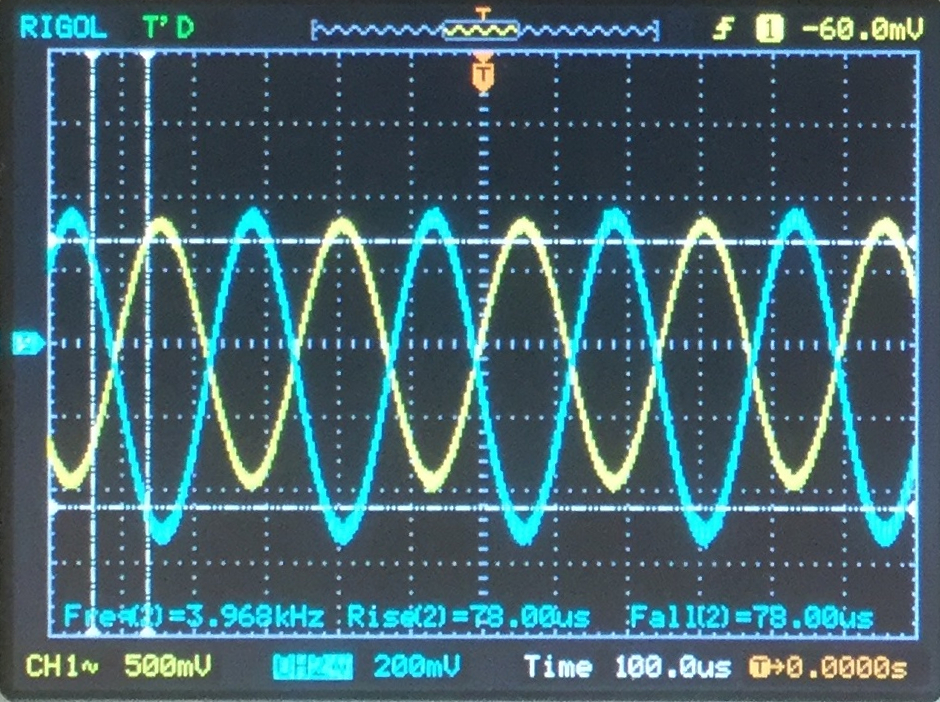
\includegraphics[width=0.5\textwidth]{czestotliwosc}
\caption{Aktualny pomiar częstotliwości badanego przebiegu}
\end{figure}
\subsection*{6.}
\begin{figure}[!h]
\centering
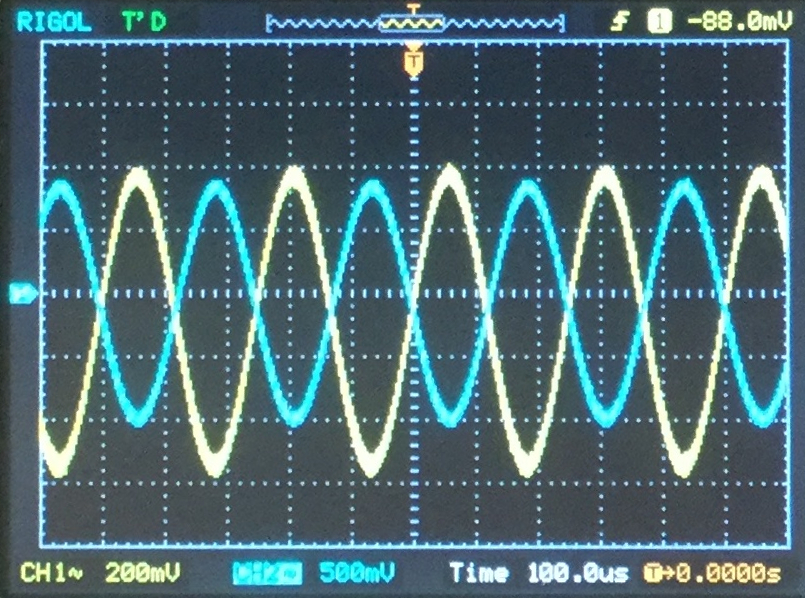
\includegraphics[width=0.5\textwidth]{k_odwracajaca}
\caption{Działanie stopnia wzmacniającego w konfiguracji odwracającej dla przełączników 1 i 1}
\end{figure}
\subsection*{7.}
Różnice zostały stwierdzone dla wzmocnienia 5,1[V/V] i są spowodowane błędem pomiaru. Szacowany błąd odczytu wartości napięcia amplitudy na oscyloskopie wynosi około 5\%% (jedna działka do wartości międzyszczytowej - 1/20), powoduje to, że wartość teoretyczna mieści się w przedziale błędu pomiaru (4,75[V/V] - 5,25[V/V]). 
\subsection*{8.}
Przesunięcie fazowe między przebiegami wynosi $180\degree$ i jest spowodowane podaniem sygnału na wejście odwracające wzmacniacza operacyjnego.


\section{Zadanie 1.5}
Badanie działania wzmacniacza całkującego (integratora)
\subsection*{3.}
Na wyjściu generatora został ustawiony przebieg prostokątny o częstotliwości 4kHz, ponieważ taka wartość została podana przez prowadzącego zajęcia.
\subsection*{4.}
\begin{figure}[!h]
\centering
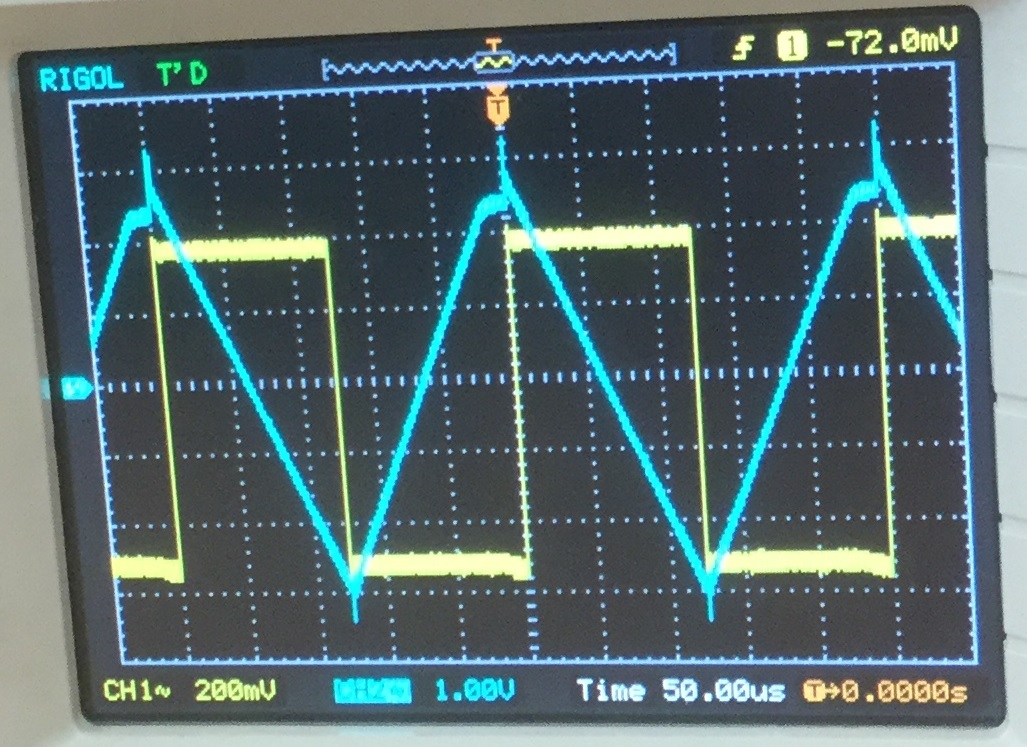
\includegraphics[width=0.5\textwidth]{przebieg_trojkatny}
\caption{Stabilny przebieg trójkątny na wyjściu integratora}
\end{figure}
\subsection*{5.}
zdjęcie i obliczenie nachylenia?????????????\\
\begin{table}[!h]
\centering
\begin{tabular}{|c|c|c|c||c|c|c|c|c|}
\hline
\textbf{$R$} & \textbf{nr przełącznika} & \textbf{$C$} & \textbf{nr przełącznika} & \textbf{$\frac{1}{T_i}$ teoretyczne} & \textbf{$\frac{1}{T_i}$ obliczone }\\ 
\hhline{|=|=|=|=#=|=|=|=|=|}
$1k\Omega$ & 1 & $10nF$ & 4 & 100000 & ???  \\
\hline
$2k\Omega$ & 2 & $10nF$ & 4 & 50000 & ???\\
\hline
\end{tabular}
\caption{Zestawienie danych pomiarowych i obliczeniowych stopnia wzmacniającego w roli integratora.}
\label{fig:dane_pomiarowe2}
\end{table}
\newpage
\subsection*{6. i 7.}
Stała całkowania i częstotliwość sygnału wejściowego zostały dobrane tak, że szerokość podstawy zbocza trójkąta pokryła się z szerokością impulsu prostokątnego.

\begin{figure}[!h]
\centering
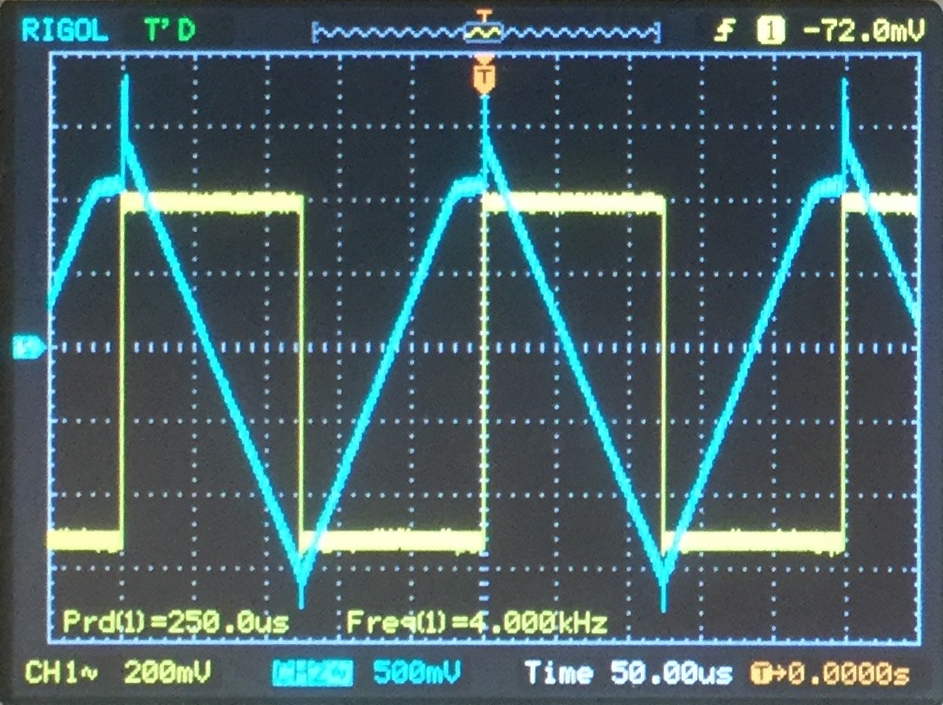
\includegraphics[width=0.5\textwidth]{czestotliwosc2}
\caption{Aktualny pomiar częstotliwości badanego przebiegu}
\end{figure}
\subsection*{8.}
\begin{figure}[!h]
\centering
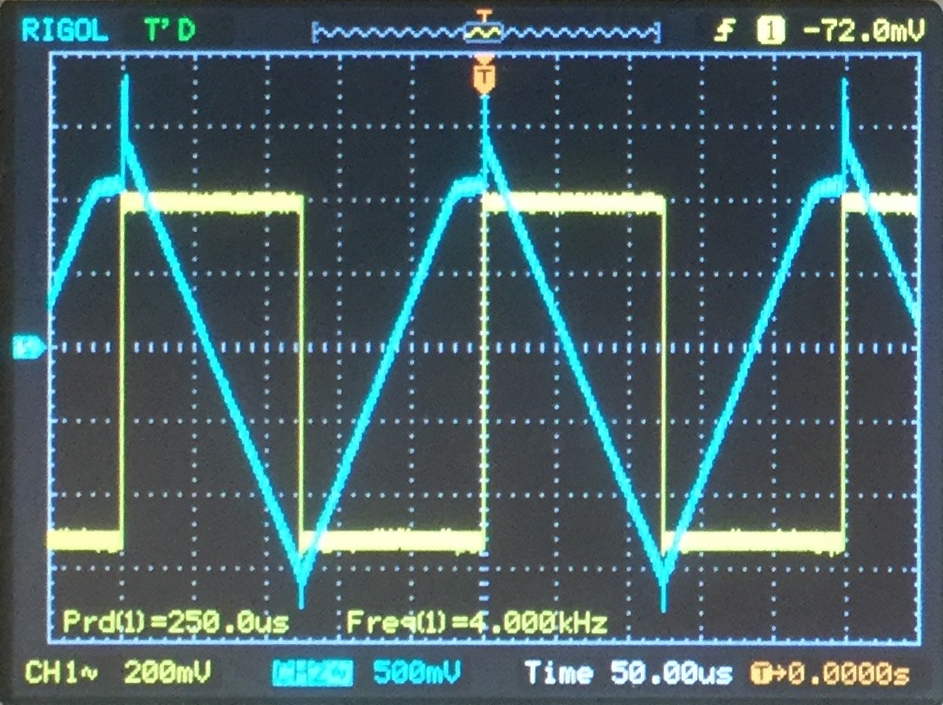
\includegraphics[width=0.5\textwidth]{czestotliwosc2}
\caption{Oscylogram ukazujący działanie integratora dla przełączników 2 i 4}
\end{figure}
\newpage
\section{Zadanie 1.6}
Badanie działania wzmacniacza różniczkującego
\subsection*{3.}
Na wyjściu generatora został ustawiony przebieg trójkątny o częstotliwości 1kHz.
\subsection*{4.}
\begin{figure}[!h]
\centering
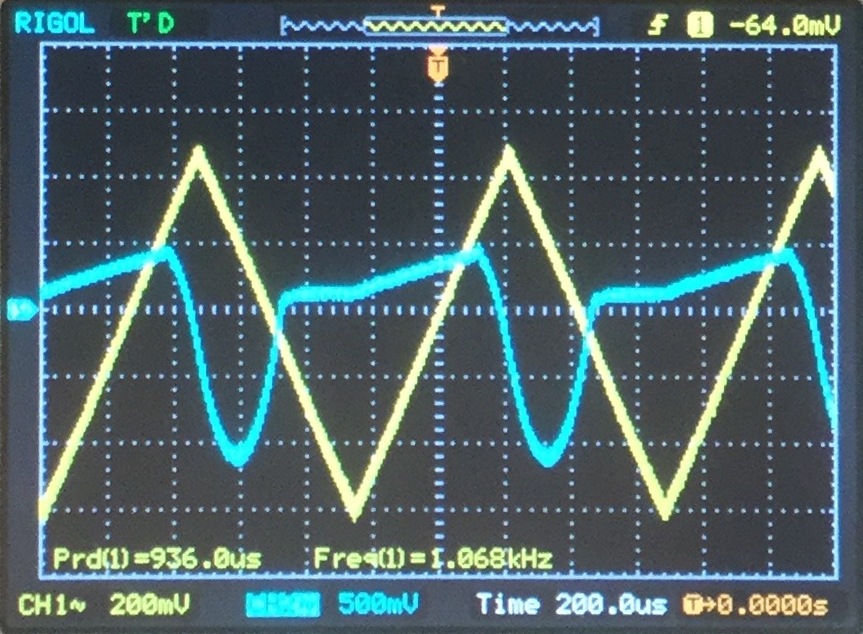
\includegraphics[width=0.5\textwidth]{czestotliwosc3}
\caption{Aktualny pomiar częstotliwości badanego przebiegu}
\end{figure}
\subsection*{5.}
\begin{figure}[!h]
\centering
\includegraphics[width=0.5\textwidth]{IMG_0310}
\caption{Stabilny przebieg prostokątny na wyjściu układu}
\end{figure}
\subsection*{6.}
\begin{figure}[!h]
\centering
\includegraphics[width=0.5\textwidth]{lepszy}
\caption{Lepszy przebieg prostokątny na wyjściu układu}
\end{figure}
\begin{figure}[!h]
\centering
\includegraphics[width=0.5\textwidth]{gorszy}
\caption{Gorszy przebieg prostokątny na wyjściu układu}
\end{figure}
\subsection*{7.}
Na przebiegu wyjściowym układu różniczkującego obserwujemy 2 rodzaje zniekształceń. Pierwsze zniekształcenie polega na ograniczonej prędkości narastania i opadania zbocza przebiegu wyjściowego. Wynika to z ograniczeń wzmacniacza operacyjnego, którego jedną z cech katalogowych jest maksymalna prędkość narastania napięcia wyjściowego (niezależne od charakterystyk częstotliwościowych). Drugie zniekształcenie wynika z pracy wzmacniacza w nasyceniu, napięcia maksymalne są równe napięciu zasilania wzmacniacza operacyjnego. Zasadniczo przebieg prostokątny otrzymano przede wszystkim ze względu na nasycenie, a w mniejszym stopniu ze względu na różniczkowanie sygnału przez układ badany.
Teoretycznie powinniśmy uzyskać zniekształcenia polegające na podwzbudzaniu wzmacniacza operacyjnego (zafalowania części płaskich) wynikające ze zbliżania się układu ze sprzeżeniem zwrotnym do stanu niestabilnego (kryterium Nyquista).


\bibliography{IEEEabrv,refs}

\begin{thebibliography}{9}

\bibitem{rlc}
  W trakcie przeprowadzania doświadczeń i pisania sprawozdania zespół korzystał głównie z materiałów ze strony http://mariusznaumowicz.ddns.net/materialy.html oraz z wiedzy własnej.\\


\end{thebibliography}

\end{document}
